\chapter{Theory}
\label{chap:theory}

\section{Sobel operator}
\label{sec:Sobel}
\paragraph*{}
The Sobel operator is used to calculate the magnitude of the image intensity gradient and thus emphasizes the edges in a given image. It is using two $3~x~3$ kernels (equation \ref{eq:sobel_calc}) to determine the horizontal ($G_x$) and vertical ($G_y$) gradients, and the Sobel output is simply the magnitude of the gradient vector.
Normally, the Euclidean distance is used to calculate the magnitude but in this assignment, the Manhattan distance will be used  as an approximation (equation \ref{eq:sobel_abs}).

\begin{equation}
\begin{array}{cc}
G_x = \left[ 
\begin{array}{ccc}
	-1 & 0 & 1\\
    -2 & 0 & 2\\
    -1 & 0 & 1\\
\end{array} \right],  &
G_y = \left[ 
\begin{array}{ccc}
	1 & 2 & 1\\
    0 & 0 & 0\\
    -1 & -2 & -1\\
\end{array}
\right]
\end{array}
\label{eq:sobel_calc}
\end{equation}\\

\begin{equation}
	Sobel = \vert G_x\vert + \vert G_y\vert
	\label{eq:sobel_abs}
\end{equation}

\paragraph*{}
If the Sobel edge detection is performed on an $8~x~6$ image as illustrated in figure \ref{fig:pic_matrix}. 
The calculation of the gradients $G_x$ and $G_y$ on the location marked by the green pixel ($A10$) is given by equation \ref{eq:sobel_Gx} and \ref{eq:sobel_Gy}.

\begin{equation}
\begin{split}
	G_x = \quad &(-1\cdot A1 ) + (0\cdot A2) + (1\cdot A3) + \\
		  &(-2\cdot A9 ) + (0\cdot A10) + (2\cdot A11)	+  \\
		  &(-1\cdot A17) + (0\cdot A18) + (1\cdot A19)
\end{split}
\label{eq:sobel_Gx}
\end{equation}

\begin{equation}
\begin{split}
	G_y = \quad & (1\cdot A1) + (2\cdot A2) + (1\cdot A3) + \\
		 &  (0\cdot A9) + (0\cdot A10) + (0\cdot A11)	+  \\
		 &  (-1\cdot A17) + (-2\cdot A18) + (-1\cdot A19)
\end{split}
\label{eq:sobel_Gy}
\end{equation}

\begin{figure}[H]
	\centering
	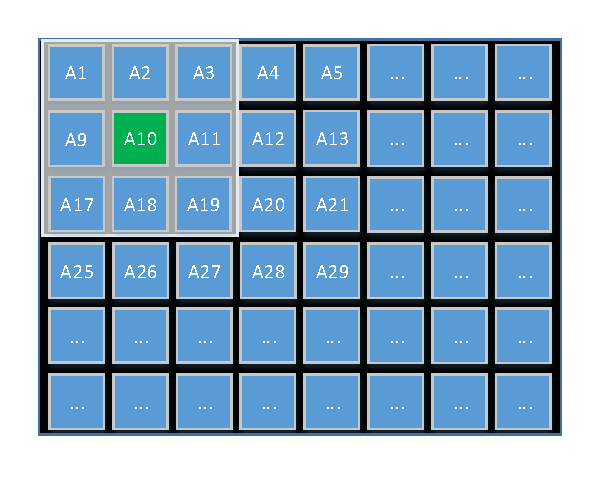
\includegraphics[width=0.5 \textwidth]{picture_example.pdf}
	\caption{Example of sobel matrix calculation}
	\label{fig:pic_matrix}
\end{figure}

\subsection{Border conditions}
\paragraph*{}
Since the Sobel operator is using a $3~x~3$ neighborhood of pixels. The processing of the image border pixels is problematic, due to the kernel being partly outside of the image. This is illustrated in figure \ref{fig:pic_matrix_border}.
There are a couple of ways to handle this border condition. One is to avoid calculation of the borders, which result in an output image that is two pixels smaller in both horizontal and vertical direction.

\begin{figure}[H]
	\centering
	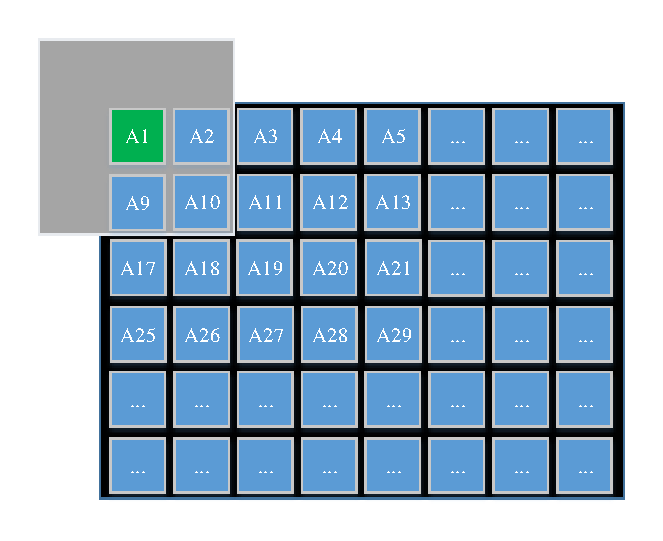
\includegraphics[width=0.5 \textwidth]{picture_example_border.pdf}
	\caption{Example of sobel matrix calculation at borders}
	\label{fig:pic_matrix_border}
\end{figure}

\paragraph*{}
A better and quite simple way to deal with the border problem is to make an imaginary or fictive border on the image. This can be done by replicating the border pixels, and use these replicated pixels to fill the kernel part that is outside of the image. This principle is illustrated in figure \ref{fig:pic_matrix_exBorder}.

\begin{figure}[H]
	\centering
	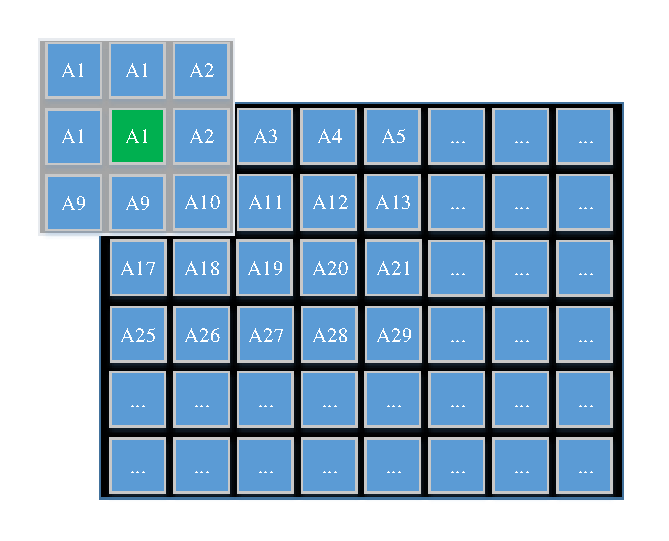
\includegraphics[width=0.5 \textwidth]{picture_example_exBorder.pdf}
	\caption{Example of sobel matrix calculation at borders}
	\label{fig:pic_matrix_exBorder}
\end{figure}  

\subsection{Dynamic range and normalization.}
\paragraph*{}
When calculating the Sobel operator, the dynamic range of the gradients $G_x$ and $G_y$, can exceed that of the input image.
For an 8-bit monochrome image, the dynamic range is [0:255], but by looking at equation \ref{eq:sobel_calc} it is clear that the  dynamic range the gradients are eight times larger [-4 $\cdot$ 255: 4 $\cdot$ 255]=[-1020: 1020]. Therefore it is required that the internal number representation, used when calculating the gradients, is sufficiently large.
For an 8-bit input image an 11 bit signed number is required. \\
The dynamic range of the Manhattan distance (equation \ref{eq:sobel_abs}) is found to be [0: 6 $\cdot$ 255] = [0:1530], which requires an 11-bit unsigned number. This range represents the highest possible gradient magnitude as illustrated by figure \ref{fig:sobel_MaxRange}.

\begin{figure}[H]
\centering
$\left[ 
\begin{array}{ccc}
	0 & 255 & 255\\
    0 & 0 & 255\\
    0 & 0 & 0\\
\end{array} \right]$
\caption{Example of maximum magnitude of gradient vector}
\label{fig:sobel_MaxRange}
\end{figure}

Since the output image is requested to be an 8-bit image, the dynamic range should be remapped from 11-bit downto 8-bit. This remapping can be done by either limiting or normalizing to the new range. In the implementations presented in this report, a normalization factor of eight is used, giving a dynamic range of [0: 191] for the Sobel output image. 


\section{Accelerator design} 
\label{sec:AccDesign}
\paragraph*{}
This section describes the design of the accelerator and explain how the pixel data is handled when travelling from external memory to the accelerator and back to external memory. 
Because each memory transaction involves two pixels (16bit data width). The proposed design of the accelerator, will process two pixels in parallel, this will increase the throughput without increasing the clock rate. At the same time it also simplifies the data handling, since the accelerator does not need to distinguish between which pixel to process (lower byte or upper byte). The drawback of this parallel approach is that the combinatorial logic that performs the Sobel operation, will be twice as big.

\paragraph*{}
As seen in the previous section \ref{sec:Sobel}, any given pixel, in the output image of the Sobel operator, is a function of the surrounding eight pixels in the input image. This requires that the accelerator is having access to these surrounding pixels, in order to evaluate the Sobel operator. Instead of reading the entire neighborhood from the external RAM, for every single pixel, an obvious improvement is to use a sliding window technique, and thereby reducing the number of memory transactions. If two pixel are to be processed in parallel, a 3x4 sliding window is required. But since the two convolution kernels stretches over three memory addresses, the width of the sliding window must be increased by one pixel, giving a total of 3x5 pixels. This is visualized in figure \ref{fig:shift_register}(a), which shows the two overlapping convolution kernels \emph{(A and B)} and the three memory location they span. \\
Figure \ref{fig:shift_register}(b) shows the proposed sliding window and illustrates how incoming pixels are shifted from right to left.

\begin{figure}[H]
	\centering
	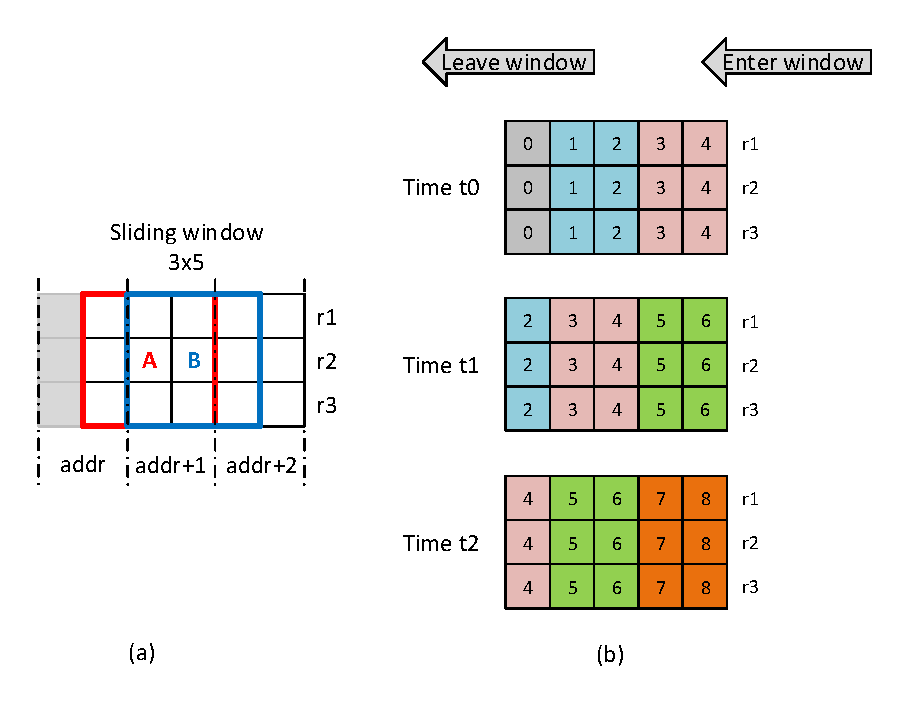
\includegraphics[width=0.9 \textwidth]{SlidingWindow.pdf}
	\caption{3x5 pixel sliding window}
	\label{fig:shift_register}
\end{figure}

\paragraph*{}
A block diagram showing the internal architecture of the accelerator is seen in figure \ref{fig:AccBlockDiagram}. The figure shows how data will flow from memory, over the sliding window through the Sobel operator and back to the memory again. A few control signals to control the memory and sliding window are also depicted in the figure. 

\begin{figure}[H]
	\centering
	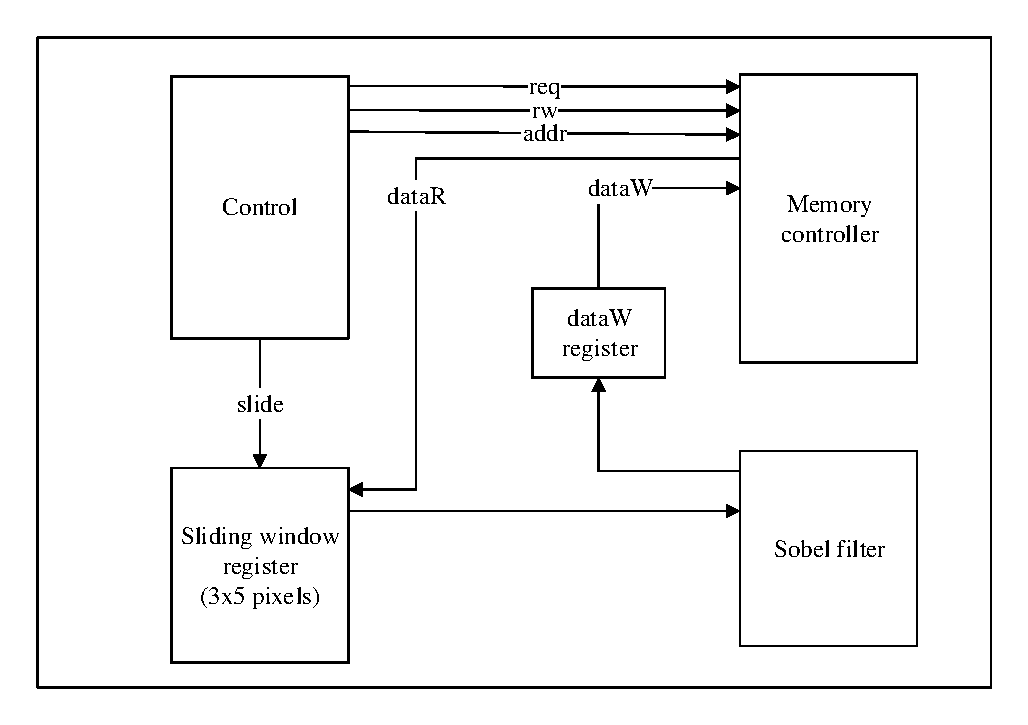
\includegraphics[width=1.0 \textwidth]{Block_diagram_overview.pdf}
	\caption{Internal architecture of the accelerator}
	\label{fig:AccBlockDiagram}
\end{figure}

\paragraph*{}
From the architecture seen in figure \ref{fig:AccBlockDiagram} along with sliding window from figure \ref{fig:shift_register} it is possible to give an initial estimate of the attainable throughput of the accelerator. For each processed pixel pair, the accelerator is required to perform three memory reads and one memory write. Because the memory controller needs to setup the address prior to reading and writing, two extra cycles are to be expected, giving a total of six clock cycles per pixel pair.
With a clock frequency of 12.5 MHz (maximum when the memory is operated in asynchronous mode \cite{Micron:CellularRAM}) this gives a throughput of approximately 4.1M pixel/sec.

\paragraph*{}
Figure \ref{fig:ASM_HW} shows a complete ASMD diagram of the proposed design, that illustrates the operation of the sliding window and details about the image border handling. The ASMD diagram consist of 9 states (\emph{idle, startRow, readSetup, readCenter, readAbove, readBelow, calculateFilter, writeData and doneImage}).
In the \emph{idle} state the accelerator is waiting for the start signal to appear. Once the start signal is detected, the state is changed to \emph{startRow}, in which the current address is initialized to the start of the current image row before entering the next state \emph{readSetup}. In the state \emph{readSetup} the reading of the current address is prepared, this state also handles the sliding of the window as well as the special case for the left and right images borders. 
The state \emph{readCenter} will put the the newly read data into the sliding window and prepare the reading of data located one row above the current position. In case of first row the top image border is handled by reading the current position once more. The state \emph{readAbove} is almost identical to \emph{readCenter}, the difference is that it will prepare the reading of data one row below the current position and that it is handling the bottom image border.
The state \emph{calculateFilter} is performing the Sobel operation and moves the result into a register. The \emph{writeData} state will write the content of the result register to the output image. From the \emph{writeData} state it is possible to enter one of three states. 1)\emph{startRow} in case the end of a row is reached. 2)\emph{doneImage} if the entire image has been processed and 3)\emph{readSetup} in the normal case.
The \emph{writeData} state will increment the current position and current row accordingly. The final state \emph{doneImage} will wait until the start signal is de-asserted before the FSM is returned to the \emph{idle} state.

\paragraph*{}
Because figure \ref{fig:ASM_HW} shows a comprehensive ASMD diagram it is possible to give a fairly accurate estimate of the registers (D-flip flop) required by the suggested design, the estimate is given in table \ref{tab:designRegisters}. 
\begin{table}[h]
	\centering
	\begin{tabular}{lr}
	\hline
	\multicolumn{2}{c}{D-flip flops registers} \\ \hline
	Register						& \# \\ \hline
	State (9 states)				& 4 \\
	3x5 pixel sliding window		& 120 \\
	Sobel result (pixel pair)		& 16 \\
	3 address registers (32 bit)	& 96 \\ \hline
	Total							& 232 \\ \hline
	\end{tabular}
	\caption{Estimated number of registers.}
	\label{tab:designRegisters}
\end{table}

\paragraph*{}
With knowledge about the arithmetic of the Sobel operator (equation \ref{eq:sobel_calc} and \ref{eq:sobel_abs} ), the required adders/subtractors can be estimated as well.
Table \ref{tab:designAdders} gives an overview of the arithmetic complexity of the accelerator design. The 7 adders stated under 'Address logic', is slightly more than the 4 adders that is directly observed from the ASMD diagram.
The 3 extra adder stems from the signals \emph{firstColumnW} and \emph{lastColoumnW}, and the calculation of the output address, which is a constant offset from the current address \emph{addr\_reg}.
 
\begin{table}[h]
	\centering
	\begin{tabular}{lr}
	\hline
	\multicolumn{2}{c}{Adders/subtractors} \\ \hline
	Function						& \# \\ \hline
	Address logic (32 bits)			& 7 \\
	Sobel filter (pixel pair, 9- 11 bits)		& 22 \\  \hline
	\end{tabular}
	\caption{Estimated number of Adders and subtractors.}
	\label{tab:designAdders}
\end{table}

\begin{figure}[H]
	\centering
	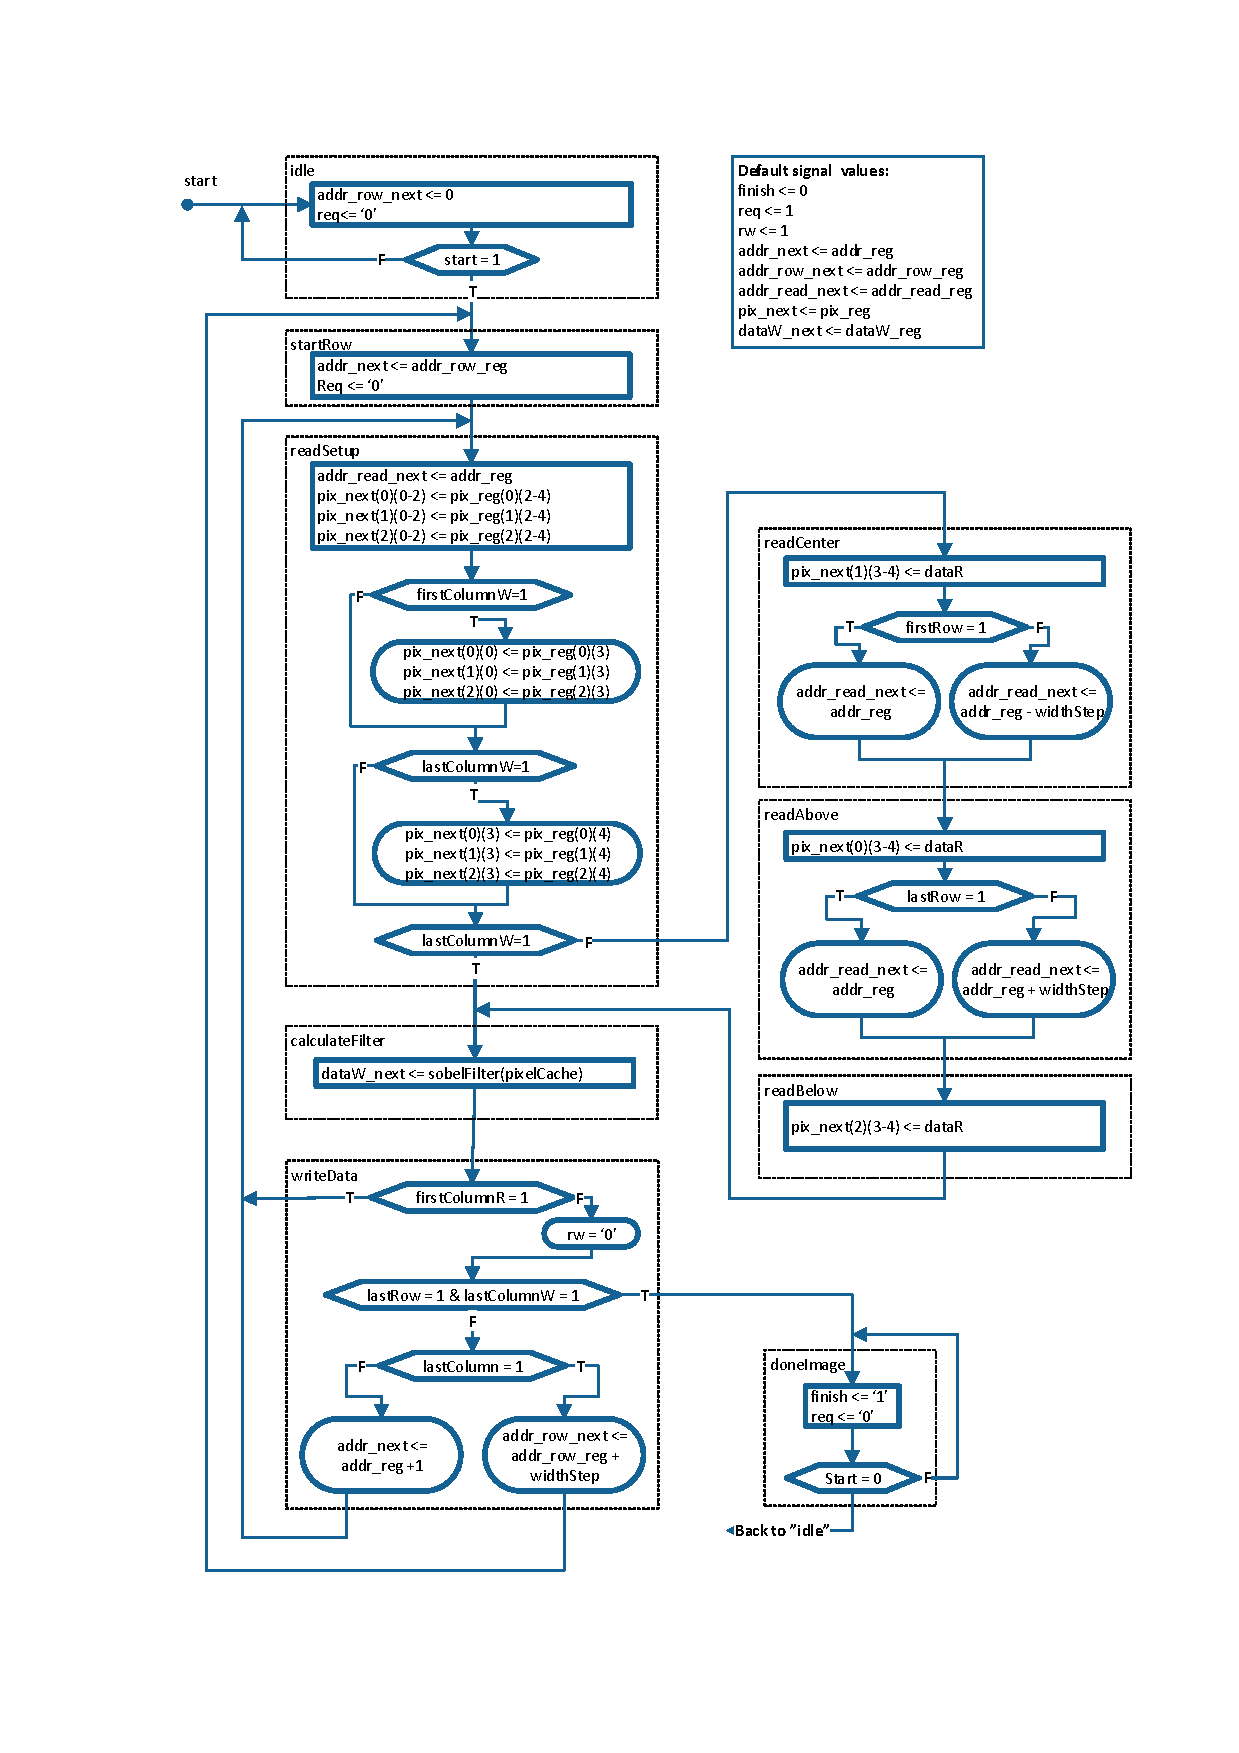
\includegraphics[width=0.95 \textwidth]{ASM_HWacc.pdf}
	\caption{ASMD chart for the edge detector hardware accelerator}
	\label{fig:ASM_HW}
\end{figure}

\section{Design optimization}
\label{sec:Optimization}
\subsection*{Removing superfluos reads}
\label{sec:memaccess}
\paragraph*{}
Even though the sliding window technique reduces the required memory transactions, the design presented in section \ref{sec:AccDesign}, still need to read every single pixel three times. This is caused by the fact that each row will need data from the row above and below the current position. Since access to the external memory is the main bottleneck in terms of achieving a high throughput, it is desirable to only read the pixel data once. By employing even more caching of data this is indeed possible. Figure \ref{fig:ScanlineBuffers} shows a caching scheme that will assure that data from three consecutive rows are available and ready to enter the sliding window. The cache operates as a delay-line buffer with one tap and contains two full scanlines. Whenever a pixel is read from the external memory it is pushed into one end of the scanline buffer and the tap and end of the delay line buffer will hold pixel data from the two rows just above the pixel being pushed into  scanline buffer. In practise the scanline buffer is implemented as a ring buffer with two pointers addressing the middle-tap and the end position. 
Incoming pixel values will overwrite the end position once it is read.

\begin{figure}[H]
	\centering
	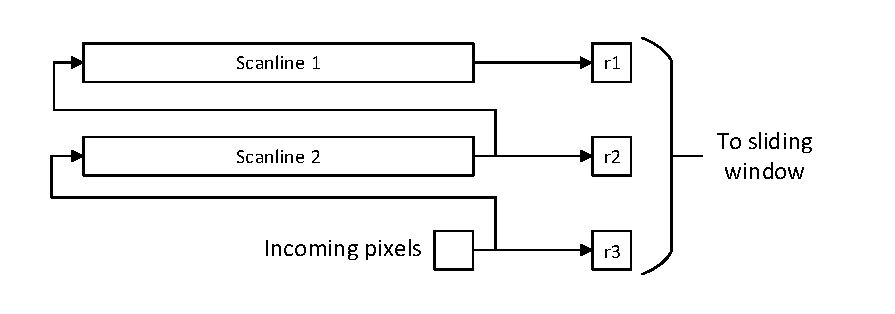
\includegraphics[width=0.9 \textwidth]{ScanlineBuffers.pdf}
	\caption{Scanline buffering of pixel data.}
	\label{fig:ScanlineBuffers}
\end{figure}

\paragraph*{}
The scanline buffer can be implemented as either distributed RAM (using LUT's) or via the block RAM, which is present on most modern FPGA's. Block RAM is usually preferred when larger memories are needed, since the distributed RAM requires more FPGA ressources. The Xilinx Spartan6 chip, used in this assignment, has a true dual ported Block RAM \cite{Xilinx:UG383}, and will be used in the implementation.
Every time the external RAM is being read, the accelerator must perform two reads and one write transaction to the block RAM. Since only two ports are available, it might seems like more than one clock cycle would be required. But because the block RAM is capable of reading the old value prior to writing the new value to a given memory location, all three transactions can be squeezed into one clock cycle.
With the addition of the scanline buffer, the optimized design is able to process a pixel pair in only two clock cycles - one is used when reading from external RAM and one when writing to the external RAM. This is three times faster, compared to a design that only use the sliding window (12.3M pixel/sec @ 12.5 MHz clock frequency)

\subsection*{Burst mode memory access}
\label{sec:burstmode}
\paragraph*{}
With the scanline buffer introduced above, each pixel is read extacly once. Hence no further throughput optimizations are possible, without increasing the clock rate. The current clock rate of 12.5MHz is limited by the asynchronous mode, that the external memory is operated under. When operating the RAM in synchronous/burst mode, a clock rate of 80MHz is attainable \cite{Micron:CellularRAM}, more than 6 times faster than the asynchronous mode.
However, the burst mode imposes a few challenges to the design, such as increased initial latency (3-4 clock cycles) and a more complex control interface. The initial latency will decrease the throughput, since switching between reading and writing bursts will add a delay to the execution. Therefore the throughput will gain by keeping the bursts as long as possible. On the other hand longer bursts requires larger internal buffering of data waiting to be written back to the RAM. Choosing a burst length of one scanline seems like a good compromise between speed and FPGA resources.

\paragraph*{}
Figure \ref{fig:ASMD_ScanlineBuffers} shows the optimized design, which implements two scanline buffers for the input data. When processing the border pixels, the design is using replication of border pixels as illustrated in figure \ref{fig:pic_matrix_exBorder}. 
Even though the design does not utilize the burst mode, it is prepared for a burst length of one scanline, by using a scanline buffer for queuing the output data, before writing to external RAM.\\
The ASMD diagram is reduced to only five states (\emph{idle}, \emph{startRow}, \emph{readData}, \emph{writeData}, \emph{doneImg}). 
The accelerator will toggle between reading and writing a full scanline. While reading a scanline from external RAM and calculating the filter result, the accelerator will stay in the state \emph{readData}. While writing the resulting scanline back to external RAM the accelerator is kept in the state \emph{writeData}.

\begin{figure}[H]
	\centering
	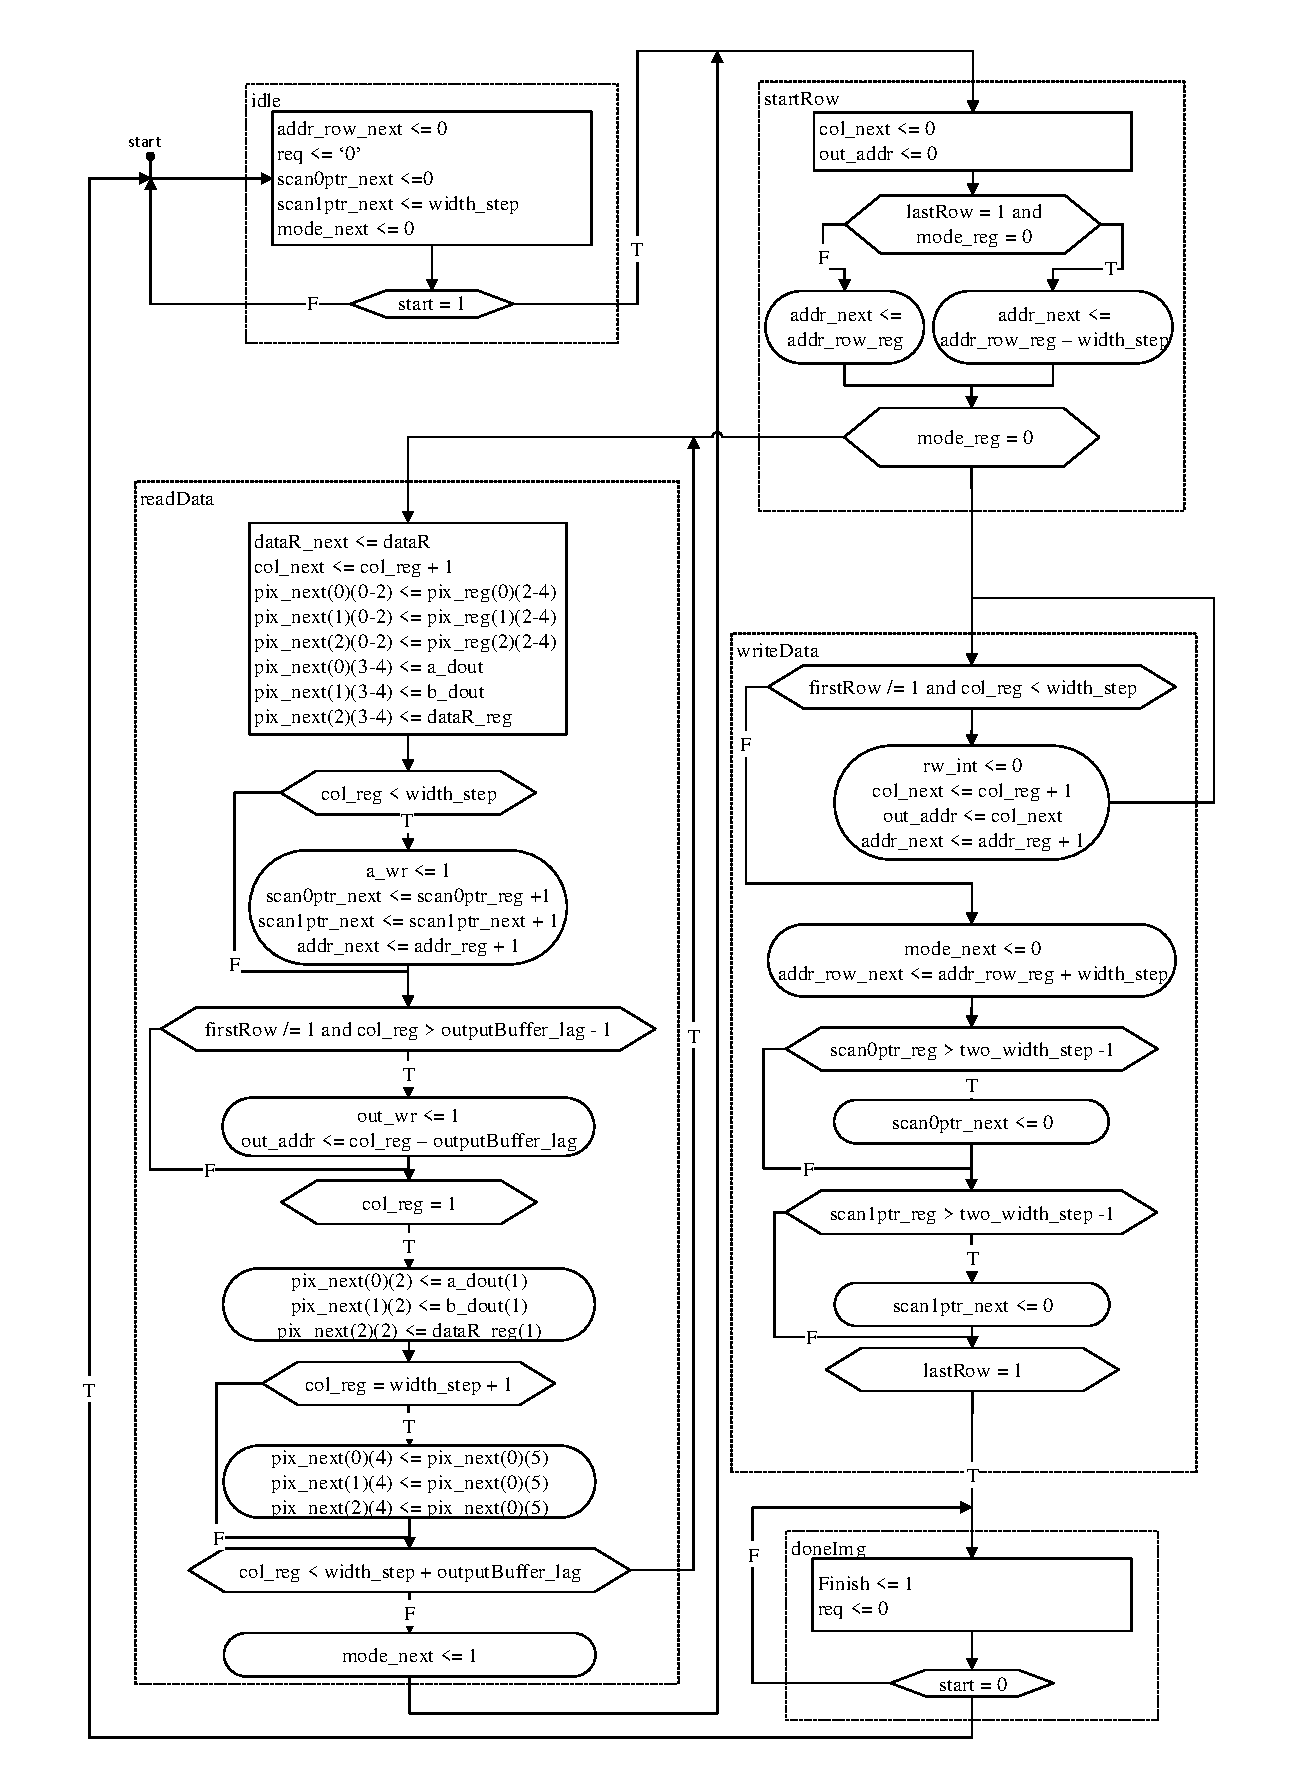
\includegraphics[width=1.0 \textwidth]{ScanlineBuffers_ASM.pdf}
	\caption{Optimized ASMD diagram with scanline buffering of pixel data.}
	\label{fig:ASMD_ScanlineBuffers}
\end{figure}
